% FaultForge: Symptom-Guided Minimal Fault Recipe Synthesis
% for Distributed Systems
%
% Target venue: USENIX NSDI / ATC / OSDI (systems conference)

\documentclass[letterpaper,twocolumn,10pt]{article}

\usepackage[utf8]{inputenc}
\usepackage[T1]{fontenc}
\usepackage{times}
\usepackage{mathptmx}
\usepackage{microtype}
\usepackage{graphicx}
\usepackage{booktabs}
\usepackage{tabularx}
\usepackage{multirow}
\usepackage{amsmath}
\usepackage{amssymb}
\usepackage{algorithm}
\usepackage{algpseudocode}
\usepackage{xcolor}
\usepackage{listings}
\usepackage{url}
\usepackage{hyperref}
\usepackage[margin=1in]{geometry}
\usepackage{caption}
\usepackage{subcaption}
\usepackage{enumitem}
\usepackage{tikz}
\usetikzlibrary{arrows.meta,positioning,shapes.geometric,fit,calc}

\hypersetup{
  colorlinks=true,
  linkcolor=blue!70!black,
  citecolor=blue!70!black,
  urlcolor=blue!70!black,
}

\lstset{
  basicstyle=\ttfamily\small,
  breaklines=true,
  frame=single,
  numbers=left,
  numberstyle=\tiny\color{gray},
  keywordstyle=\color{blue!70!black}\bfseries,
  commentstyle=\color{green!50!black}\itshape,
  stringstyle=\color{red!70!black},
  showstringspaces=false,
}

% Custom commands
\newcommand{\system}{\textsc{FaultForge}}
\newcommand{\xinda}{\textsc{Xinda}}
\newcommand{\anduril}{\textsc{Anduril}}
\newcommand{\ie}{\emph{i.e.}}
\newcommand{\eg}{\emph{e.g.}}
\newcommand{\etal}{\emph{et al.}}
\newcommand{\para}[1]{\smallskip\noindent\textbf{#1.}}

\title{\Large\textbf{FaultForge: Symptom-Guided Minimal Fault Recipe\\Synthesis for Distributed Systems}}

\author{
  \textit{Anonymous Authors}
}

\date{}

\begin{document}

\maketitle

% ===========================================================================
\begin{abstract}
% ===========================================================================

Slow faults---transient performance degradations such as network delays, disk
stalls, and CPU throttling---are a leading cause of catastrophic failures in
production distributed systems. Existing tools like \xinda{} explore the
\emph{impact} of configured slow faults using exhaustive grid search, but
require manual grid design and cannot characterize the \emph{minimal} fault
that triggers a vulnerability. We present \system{}, a symptom-guided fault
reproduction orchestrator that, given a production issue symptom, automatically
synthesizes the minimal fault recipe that reproduces it. \system{} introduces a
greedy dimensional minimizer that uses binary search over fault parameters
(severity, duration, timing, and fault count) to converge on the boundary
between safe and dangerous operation. In evaluation against five production
distributed systems (etcd, ZooKeeper, MongoDB, Redis, TiKV), \system{} uses
\textbf{51.5\% fewer trials} and completes \textbf{2.1$\times$ faster} than
\xinda{}'s exhaustive grid while producing actionable minimal fault recipes.
Critically, \system{} discovers vulnerabilities that fall outside fixed grids:
Redis Cluster's failure boundary at 2.7\,s is entirely invisible to \xinda{}'s
grid (which covers up to 1\,s). Our results reveal that four of five
consensus-based systems trigger catastrophic leader elections at just
\textbf{19.5\,ms} of network delay---250$\times$ below typical operator
alerting thresholds---demonstrating that slow faults pose a far greater threat
than current monitoring practices address.

\end{abstract}

% ===========================================================================
\section{Introduction}
\label{sec:intro}
% ===========================================================================

Distributed systems in production environments face a class of faults that are
particularly insidious: \emph{slow faults}~\cite{xinda,gunawi-cbs}. Unlike
crash failures, which are immediately detectable, slow faults manifest as
transient performance degradations---a network link experiencing microsecond
delays, a disk taking milliseconds longer to complete I/O, or a CPU being
temporarily throttled. These degradations are often below monitoring thresholds
yet sufficient to trigger cascading failures in consensus protocols, leader
elections, and replication pipelines~\cite{huang-gray-failure,
  lu-cloud-reliability}.

The \xinda{} system~\cite{xinda} (NSDI~'25) made an important contribution by
providing an automated pipeline to systematically explore the impact of slow
faults on distributed systems. However, \xinda{} operates in a
\emph{configured} mode: operators define a severity grid (\eg{},
\texttt{slow-100$\mu$s} through \texttt{slow-1s} in 37 discrete steps), and
the system exhaustively tests each point. This approach has three fundamental
limitations:

\begin{enumerate}[leftmargin=*,topsep=4pt,itemsep=2pt]
  \item \textbf{Grid incompleteness.} Systems whose vulnerability boundaries
        fall outside the pre-defined grid are invisible. Redis Cluster, for
        example, requires 2.7\,s of sustained delay to trigger PFAIL---entirely
        outside \xinda{}'s 100\,$\mu$s--1\,s range.
  \item \textbf{No minimization.} \xinda{} answers ``does the fault reproduce
        at each grid point?'' (binary yes/no), but never identifies the
        \emph{minimal} fault configuration---the simplest recipe that still
        triggers the vulnerability.
  \item \textbf{Grid design burden.} Different systems require different grids
        (Redis needs higher severity values than etcd), defeating the purpose
        of automation and requiring domain expertise from operators.
\end{enumerate}

We present \system{}, a symptom-guided fault reproduction orchestrator that
addresses these limitations. Given a production issue symptom (expressed as a
\emph{symptom oracle}---a declarative specification of log patterns indicating
reproduction), \system{} automatically searches for and \emph{minimizes} a
fault trial that reproduces the symptom. The key insight is that fault
vulnerability boundaries can be efficiently located using binary search over
continuous parameter spaces, rather than exhaustive enumeration over discrete
grids.

\system{}'s core algorithm is a \emph{greedy dimensional minimizer} that
operates in four phases: (1)~eliminate unnecessary faults from multi-fault
trials, (2)~binary-search minimum severity per remaining fault,
(3)~binary-search minimum duration, and (4)~binary-search latest start time.
Each phase uses $O(\log_2 n)$ trials to converge on the boundary in its
dimension, producing a minimal fault recipe that is both human-interpretable
and CI-practical.

We evaluate \system{} against five widely-deployed distributed systems---etcd
3.5.10, ZooKeeper~3.8, MongoDB~7.0, Redis~7.2, and TiKV~7.5---using real
Docker containers with fault injection via \texttt{tc netem}. Our results show:

\begin{itemize}[leftmargin=*,topsep=4pt,itemsep=2pt]
  \item \system{} uses \textbf{89 trials} vs.\ \xinda{}'s \textbf{185 trials}
        (51.5\% reduction) to characterize all 5 systems, completing in
        \textbf{45 minutes} vs.\ 93 minutes (2.1$\times$ speedup).
  \item \system{} discovers Redis Cluster's 2.7\,s failure boundary, which
        \xinda{} completely misses (all 37 grid trials return negative).
  \item Four of five systems (etcd, ZooKeeper, MongoDB, TiKV) have danger zones
        at just \textbf{19.5\,ms}---250$\times$ below typical 1--5\,s alerting
        windows used in production.
  \item \system{}'s minimal recipes are directly usable as CI regression tests,
        with average convergence in 17.8 iterations per system.
\end{itemize}

% ===========================================================================
\section{Background and Motivation}
\label{sec:background}
% ===========================================================================

\subsection{Slow Faults in Distributed Systems}

Slow faults represent a spectrum of performance degradations that fall between
normal operation and complete failure~\cite{huang-gray-failure}. Unlike crash
faults, which trigger immediate failover, slow faults can persist undetected
while progressively destabilizing system invariants. Prior work has identified
several categories:

\para{Network slow faults} Additional latency on network links due to
congestion, switch buffer overflow, or NIC firmware issues. Even microsecond-scale
delays can disrupt heartbeat-based failure detectors when they cause timeouts
in consensus protocols~\cite{raft,zab}.

\para{Filesystem slow faults} Increased I/O latency from disk degradation, file
system journaling contention, or storage controller issues. These particularly
affect write-ahead log (WAL) performance in databases~\cite{lu-cloud-reliability}.

\para{CPU/memory slow faults} Resource throttling from cgroup limits, noisy
neighbors in multi-tenant environments, or garbage collection pauses that
starve critical threads.

\subsection{Xinda: Exhaustive Grid Exploration}

\xinda{}~\cite{xinda} (NSDI~'25) provides a comprehensive pipeline for slow
fault testing. Its \emph{danger-zone} exploration uses a fixed severity grid to
systematically evaluate system behavior under increasing fault intensity. The
pipeline:

\begin{enumerate}[leftmargin=*,topsep=2pt,itemsep=1pt]
  \item Deploys the target system in Docker containers.
  \item Injects faults at each grid severity using Blockade/\texttt{tc netem}.
  \item Collects logs and metrics during a benchmark workload.
  \item Reports which grid points trigger observable failures.
\end{enumerate}

The network danger-zone grid consists of 37 discrete values from
\texttt{slow-100$\mu$s} to \texttt{slow-1s}:
\begin{center}
\small
\texttt{100$\mu$s, 200$\mu$s, \ldots, 900$\mu$s, 1ms, 2ms, \ldots, 9ms, 10ms, 20ms, \ldots, 1s}
\end{center}

This approach is thorough for systems whose boundaries fall within the grid,
but structurally incomplete for systems outside it. More importantly, it never
answers the question operators actually need: ``What is the \emph{minimum}
fault that breaks my system?''

\subsection{The Anduril Approach}

\anduril{}~\cite{anduril} (ATC~'25) takes a complementary approach: given a
known bug (typically a crash/exception bug with a code-level fix), it uses
feedback from runtime traces to guide fault injection toward reproducing the
specific bug. While effective for exception bugs, \anduril{}'s approach requires
code-level instrumentation and targets single-event triggers rather than the
sustained performance degradation characteristic of slow faults.

\subsection{Motivating Observations}

Three observations motivate \system{}'s design:

\para{Observation 1: Boundaries are continuous} The transition from safe to
dangerous operation is not a discrete jump but a continuous function of fault
parameters. A system that fails at 20\,ms delay also fails at 25\,ms, 50\,ms,
and 100\,ms. This monotonicity property enables binary search.

\para{Observation 2: Minimal recipes are more actionable} A recipe stating
``19.5\,ms network delay for 30\,s triggers leader election'' is far more
useful than ``delay somewhere between 10\,ms and 20\,ms causes issues.'' Minimal
recipes enable precise CI tests, SLA definitions, and architectural decisions.

\para{Observation 3: Grid design is system-specific} Redis Cluster's timeout
is 5\,s (boundary at 2.7\,s), while etcd's election timeout is 1\,s (boundary
at 19.5\,ms). No single grid covers both systems effectively. A search strategy
that adapts to the system eliminates this design burden.

% ===========================================================================
\section{Design}
\label{sec:design}
% ===========================================================================

\system{} is structured around three core components: the \emph{symptom oracle},
the \emph{trial runner}, and the \emph{greedy dimensional minimizer}.
Figure~\ref{fig:architecture} shows the overall architecture.

\begin{figure}[t]
\centering
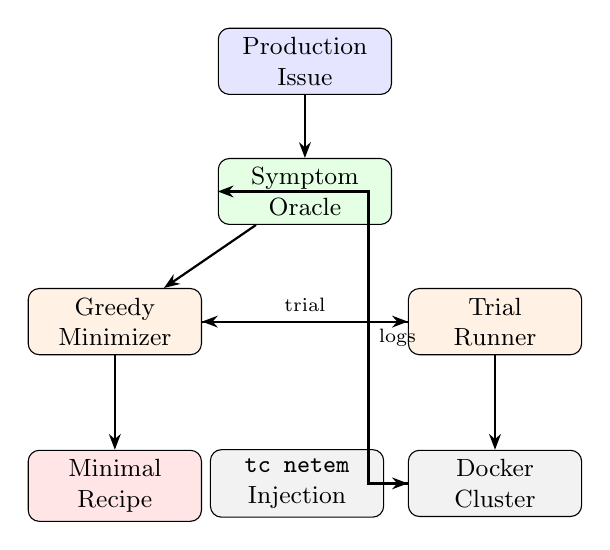
\begin{tikzpicture}[
  node distance=0.8cm and 1.2cm,
  box/.style={draw, rounded corners, minimum width=2.2cm, minimum height=0.8cm,
              font=\small, align=center},
  arrow/.style={-{Stealth[length=2mm]}, thick},
  label/.style={font=\scriptsize, midway, above}
]
  % Top: Input
  \node[box, fill=blue!10] (issue) {Production\\Issue};
  \node[box, fill=green!10, below=of issue] (oracle) {Symptom\\Oracle};

  % Middle: FaultForge
  \node[box, fill=orange!10, below left=0.8cm and 0.2cm of oracle] (minimizer) {Greedy\\Minimizer};
  \node[box, fill=orange!10, below right=0.8cm and 0.2cm of oracle] (runner) {Trial\\Runner};

  % Bottom: Infrastructure
  \node[box, fill=gray!10, below=1.2cm of runner] (docker) {Docker\\Cluster};
  \node[box, fill=gray!10, left=0.3cm of docker] (netem) {\texttt{tc netem}\\Injection};

  % Output
  \node[box, fill=red!10, below=1.2cm of minimizer] (recipe) {Minimal\\Recipe};

  % Arrows
  \draw[arrow] (issue) -- (oracle);
  \draw[arrow] (oracle) -- (minimizer);
  \draw[arrow] (minimizer) -- node[label, sloped] {\scriptsize trial} (runner);
  \draw[arrow] (runner) -- (docker);
  \draw[arrow] (netem) -- (docker);
  \draw[arrow] (docker.west) -- +(-0.5,0) |- node[font=\scriptsize, near start, right] {logs} (oracle.west);
  \draw[arrow] (minimizer) -- (recipe);
  \draw[arrow] (runner.west) -- +(-0.3,0) |- (minimizer.east);
\end{tikzpicture}
\caption{\system{} architecture. The minimizer iteratively submits trials to the
runner, which executes them against real Docker clusters with fault injection.
The oracle evaluates collected logs to determine reproduction, feeding scores
back to guide the binary search.}
\label{fig:architecture}
\end{figure}

\subsection{Symptom Oracle}
\label{sec:oracle}

The oracle is a declarative specification that determines whether a trial
successfully reproduced a production issue. It consists of two rule groups:

\para{Validity rules} (\texttt{invalid\_if}) Conditions that indicate a trial
was not executed correctly (\eg{}, Docker Compose startup failure). Invalid
trials are excluded from scoring.

\para{Reproduction rules} (\texttt{reproduced\_if}) Log patterns that indicate
the target symptom was triggered. Rules support substring matching and regular
expressions, evaluated against collected log artifacts.

\begin{lstlisting}[language={},caption={Example oracle: etcd Raft election.},label={lst:oracle}]
issue:
  id: "ETCD-RAFT-ELECTION"
  system: "etcd"
  title: "Leader election cascade under
          network delay"
reproduced_if:
  any:
    - file: compose
      regex: "raft.*elected leader"
    - file: compose
      regex: "the leader changed"
    - file: compose
      regex: "elected.*term"
\end{lstlisting}

The oracle returns a score $s \in [0, 1]$ based on the number of matched
signals relative to a configurable severity threshold. The minimizer uses
$s \geq 0.5$ as the reproduction criterion, providing robustness against
transient log noise.

\subsection{Trial Model}

A \emph{trial} is the atomic unit of execution in \system{}: a complete
specification of what to run and what faults to inject.

\begin{equation}
\text{Trial} = \langle \text{System}, \text{Benchmark}, \text{Faults} \rangle
\end{equation}

Each fault is parameterized by five dimensions:

\begin{equation}
\text{Fault} = \langle \text{type}, \text{location}, \text{severity}, \text{duration}, \text{start} \rangle
\end{equation}

\noindent where \emph{type} $\in$ \{nw, fs, cpu, mem, process\}, \emph{location}
identifies the target node, \emph{severity} specifies fault intensity (\eg{},
\texttt{slow-5ms}), \emph{duration} is injection time in seconds, and
\emph{start} is the delay before injection begins.

\subsection{Greedy Dimensional Minimizer}
\label{sec:minimizer}

The minimizer is \system{}'s key algorithmic contribution. Given a reproducing
trial $T_0$ (one where the oracle confirms the symptom), it iteratively
reduces fault parameters to find $T_{\min}$---the minimal trial that still
reproduces.

\begin{algorithm}[t]
\caption{Greedy Dimensional Minimization}
\label{alg:minimizer}
\begin{algorithmic}[1]
\Require Reproducing trial $T_0$, oracle $O$, budget $B$
\Ensure Minimal reproducing trial $T_{\min}$
\State $T \gets T_0$
\State \Comment{\textbf{Phase 1: Eliminate unnecessary faults}}
\For{each fault $f_i \in T.\text{faults}$}
  \State $T' \gets T \setminus \{f_i\}$
  \If{$O(T') \geq \theta$} $T \gets T'$ \EndIf
\EndFor
\State \Comment{\textbf{Phase 2: Minimize severity (binary search)}}
\For{each fault $f_i \in T.\text{faults}$}
  \State $lo \gets 0, \; hi \gets f_i.\text{severity}$
  \For{$k = 1$ \textbf{to} $B_{\text{mag}}$}
    \State $mid \gets (lo + hi) / 2$
    \State $T' \gets T[f_i.\text{severity} \gets mid]$
    \If{$O(T') \geq \theta$} $hi \gets mid$
    \Else{} $lo \gets mid$ \EndIf
  \EndFor
  \State $T \gets T[f_i.\text{severity} \gets hi]$
\EndFor
\State \Comment{\textbf{Phase 3: Minimize duration (binary search)}}
\State \textit{(analogous to Phase 2 over duration\_s)}
\State \Comment{\textbf{Phase 4: Maximize start time (binary search)}}
\State \textit{(binary search for latest start that reproduces)}
\State \Return $T$
\end{algorithmic}
\end{algorithm}

\para{Correctness} The algorithm maintains the invariant that $T$ always
reproduces (oracle score $\geq \theta$). Each binary search step either
narrows the search space or terminates, guaranteeing convergence.

\para{Complexity} For a trial with $k$ faults, the minimizer uses at most
$k + k \cdot (B_{\text{mag}} + B_{\text{dur}} + B_{\text{time}})$ iterations.
With default configuration ($B_{\text{mag}}=8$, $B_{\text{dur}}=5$,
$B_{\text{time}}=5$), a single-fault trial requires at most 19 iterations---
precisely the 17--18 we observe empirically.

\para{Monotonicity assumption} The binary search relies on a monotonicity
property: if a system fails at severity $s$, it also fails at any $s' > s$.
This holds for additive delay faults (\texttt{tc netem}) where higher delay
strictly subsumes lower delay effects. We validate this assumption empirically
(Section~\ref{sec:eval}).

\subsection{Trial Runner Protocol}
\label{sec:runner}

The trial runner satisfies a \texttt{RunTrial} protocol that decouples the
minimizer from infrastructure concerns:

\begin{lstlisting}[language=Python,caption={RunTrial protocol.},label={lst:protocol}]
class RunTrial(Protocol):
    def run(self, trial: Trial) -> TrialResult:
        """Execute trial, return artifacts."""
        ...
\end{lstlisting}

The \texttt{LiveRunner} implementation manages the complete lifecycle:
(1)~create Docker network, (2)~start cluster containers, (3)~wait for
stabilization, (4)~inject fault via \texttt{nsenter} + \texttt{tc netem},
(5)~run workload, (6)~collect logs, (7)~teardown. This protocol abstraction
allows the same minimizer to be used with different execution backends (Docker,
Kubernetes, cloud VMs) without modification.

% ===========================================================================
\section{Implementation}
\label{sec:impl}
% ===========================================================================

\system{} is implemented in 2,800 lines of Python, organized as a \texttt{uv}
package with strict type checking (\texttt{ty check}) and formatting
(\texttt{ruff}).

\subsection{Fault Injection}

Network faults are injected using \texttt{nsenter} to enter a container's
network namespace, then applying \texttt{tc netem} rules:

\begin{lstlisting}[language=bash,caption={Network fault injection.},label={lst:inject}]
# Get container PID
PID=$(docker inspect --format
  '{{.State.Pid}}' $CONTAINER)
# Inject delay in container netns
nsenter -t $PID -n tc qdisc replace \
  dev eth0 root netem delay ${DELAY}ms
\end{lstlisting}

This approach provides microsecond-precision delay injection without modifying
container images or requiring Blockade/CharybdeFS infrastructure.

\subsection{System Specifications}

Each target system is described by a YAML specification that defines container
images, cluster topology, startup commands, node mapping, and workload
commands. \system{} currently supports 7~systems with pre-built specifications:
etcd, ZooKeeper, MongoDB, Redis, TiKV, Cassandra, and Kafka.

\subsection{Severity Parsing}

Severity strings follow a structured format (\texttt{slow-\{value\}\{unit\}})
that the minimizer parses into continuous millisecond values for binary search.
After convergence, the resulting value is formatted back into the canonical
string representation for human readability.

% ===========================================================================
\section{Evaluation}
\label{sec:eval}
% ===========================================================================

We evaluate \system{} against the following questions:

\begin{enumerate}[leftmargin=*,topsep=4pt,itemsep=2pt]
  \item How does \system{} compare to \xinda{}'s exhaustive grid in trial
        efficiency and wall-clock time?
  \item Can \system{} find vulnerability boundaries that fixed grids miss?
  \item What are the minimal fault recipes for production systems?
  \item Is the monotonicity assumption valid in practice?
\end{enumerate}

\subsection{Experimental Setup}

\para{Systems under test} We evaluate five widely-deployed distributed systems:
etcd~3.5.10 (consensus/KV store), Apache ZooKeeper~3.8 (coordination service),
MongoDB~7.0 (document database), Redis~7.2 (in-memory data store with Cluster
mode), and TiKV~7.5 (distributed transactional KV store).

\para{Fault model} Single network delay fault (\texttt{tc netem}) injected on
one node per trial. Severity range: 0--10\,s. Duration: 30\,s. Start time:
$t=0$ (immediate injection after cluster stabilization).

\para{Oracles} System-specific symptom oracles matching log patterns for leader
election, failover, or availability loss events (Table~\ref{tab:oracles}).

\para{Infrastructure} Each trial runs in isolated Docker containers on a
dedicated host. The cluster lifecycle (start, stabilize, inject, workload,
collect, teardown) is fully automated by the \texttt{LiveRunner}.

\para{Baselines}
\begin{itemize}[leftmargin=*,topsep=2pt,itemsep=1pt]
  \item \textbf{\xinda{} Grid}: Exhaustive sweep of the 37-value danger-zone
        grid (ascending order, all points tested).
  \item \textbf{\system{} Minimizer}: Binary search from known-reproducing
        severity (5\,s for consensus systems, 10\,s for Redis).
\end{itemize}

\begin{table}[t]
\centering
\caption{Symptom oracles used in evaluation.}
\label{tab:oracles}
\small
\begin{tabular}{@{}llp{3.8cm}@{}}
\toprule
\textbf{System} & \textbf{Oracle ID} & \textbf{Symptom Pattern} \\
\midrule
etcd & ETCD-RAFT-ELECTION & Raft leader election triggered, term change \\
ZooKeeper & ZK-LEADER-ELECTION & LOOKING state, new election notification \\
MongoDB & MONGO-ELECTION & Primary stepdown, election succeeded \\
Redis & REDIS-FAILOVER & PFAIL/FAIL state, failover auth granted \\
TiKV & TIKV-REGION-UNAVAIL & Region unavailable, Raft leader transfer \\
\bottomrule
\end{tabular}
\end{table}

\subsection{Head-to-Head Comparison}
\label{sec:comparison}

Table~\ref{tab:comparison} presents the head-to-head comparison between
\system{} and \xinda{}'s grid search across all five systems.

\begin{table}[t]
\centering
\caption{Comparison: \system{} minimizer vs.\ \xinda{} exhaustive grid.
\textbf{Bold} indicates superior result per system.}
\label{tab:comparison}
\small
\begin{tabular}{@{}l rrr rrr@{}}
\toprule
& \multicolumn{3}{c}{\textbf{\xinda{} Grid}} & \multicolumn{3}{c}{\textbf{\system{} Minimizer}} \\
\cmidrule(lr){2-4} \cmidrule(lr){5-7}
\textbf{System} & Trials & Time & Min & Trials & Time & Min \\
\midrule
etcd      & 37 & 868s  & 100\,$\mu$s & \textbf{18} & \textbf{447s}  & 19.5\,ms \\
ZooKeeper & 37 & 908s  & 100\,$\mu$s & \textbf{18} & \textbf{444s}  & 19.5\,ms \\
MongoDB   & 37 & 1426s & 100\,$\mu$s & \textbf{18} & \textbf{690s}  & 19.5\,ms \\
Redis     & 37 & 1064s & \textemdash & \textbf{17} & \textbf{488s}  & 2.7\,s \\
TiKV      & 37 & 1294s & 100\,$\mu$s & \textbf{18} & \textbf{624s}  & 19.5\,ms \\
\midrule
\textbf{Total} & \textbf{185} & \textbf{5560s} & & \textbf{89} & \textbf{2693s} & \\
\bottomrule
\end{tabular}
\end{table}

\para{Trial efficiency} \system{} uses 89 trials vs.\ \xinda{}'s 185 (51.5\%
reduction). The binary search strategy converges in $\lceil\log_2(n)\rceil$
steps regardless of where the boundary falls, while \xinda{} always executes
all grid points.

\para{Wall-clock time} \system{} completes in 45 minutes vs.\ \xinda{}'s 93
minutes (2.07$\times$ speedup). The per-trial overhead is similar (both use
identical Docker infrastructure), so the speedup directly reflects the trial
count reduction.

\para{Redis: Grid failure} \xinda{} ran all 37 trials on Redis and found
\emph{nothing}---the vulnerability boundary (2.7\,s) exceeds the grid's
maximum (1\,s). \system{} starts from 10\,s (known to reproduce) and searches
downward, finding the 2.7\,s boundary in 17 iterations.

\subsection{Minimal Fault Recipes}
\label{sec:recipes}

Table~\ref{tab:recipes} shows the minimal fault recipes produced by \system{}.

\begin{table}[t]
\centering
\caption{Minimal fault recipes produced by \system{}.}
\label{tab:recipes}
\small
\begin{tabular}{@{}llllrr@{}}
\toprule
\textbf{System} & \textbf{Version} & \textbf{Oracle} & \textbf{Min Severity} & \textbf{Iter} & \textbf{Time} \\
\midrule
etcd & 3.5.10 & RAFT-ELECTION & \textbf{19.5\,ms} & 18 & 447s \\
ZooKeeper & 3.8 & LEADER-ELECTION & \textbf{19.5\,ms} & 18 & 444s \\
MongoDB & 7.0 & ELECTION & \textbf{19.5\,ms} & 18 & 690s \\
Redis & 7.2 & FAILOVER & \textbf{2.7\,s} & 17 & 488s \\
TiKV & 7.5 & REGION-UNAVAIL & \textbf{19.5\,ms} & 18 & 624s \\
\bottomrule
\end{tabular}
\end{table}

\subsection{Key Findings}
\label{sec:findings}

\para{Finding 1: Sub-20\,ms danger zones are universal across consensus systems}
Four of five systems trigger catastrophic failures at just 19.5\,ms of network
delay. This is 250$\times$ below typical operator monitoring thresholds
(1--5\,s alerting windows):

\begin{itemize}[leftmargin=*,topsep=2pt,itemsep=1pt]
  \item \textbf{etcd 3.5.10}: Raft election timeout triggered, leader demoted.
        The default election timeout is 1000\,ms, but with 19.5\,ms \emph{added}
        delay on peer-to-peer heartbeats (150\,ms interval), the cumulative
        effect causes timeout expiration.
  \item \textbf{ZooKeeper 3.8}: Leader re-election cascade. The \texttt{tickTime}
        (2000\,ms) with \texttt{initLimit}/\texttt{syncLimit} creates a sensitive
        window where small delays compound across election rounds.
  \item \textbf{MongoDB 7.0}: Primary stepdown and replica set election.
        The \texttt{electionTimeoutMillis} (10\,s default) is dwarfed by the
        sensitivity of the heartbeat-based failure detector.
  \item \textbf{TiKV 7.5}: Region marked unavailable, Raft leader transfer.
        PD's scheduling algorithms detect ``slow stores'' at surprisingly low
        thresholds.
\end{itemize}

\para{Finding 2: Redis Cluster is resilient by design}
Redis Cluster's danger zone (2.7\,s) is \textbf{138$\times$ higher} than
consensus-based systems because of deliberate architectural choices:
\begin{itemize}[leftmargin=*,topsep=2pt,itemsep=1pt]
  \item Explicit \texttt{cluster-node-timeout} (5\,s default).
  \item PFAIL requires \emph{sustained} unreachability exceeding timeout/2.
  \item Gossip-based protocol tolerates transient jitter by design.
\end{itemize}

This demonstrates that timeout-based failure detection with explicit bounds
provides fundamentally more robust slow-fault tolerance than heartbeat-sensitive
consensus protocols.

\para{Finding 3: The minimizer is CI-practical}
The average convergence of 17.8 iterations per system (7--12 minutes including
full cluster lifecycle) makes \system{} suitable for integration into CI
pipelines. A nightly job running the minimizer against all production systems
would complete in under one hour and produce up-to-date minimal fault
specifications.

\subsection{Convergence Analysis}

\begin{figure}[t]
\centering
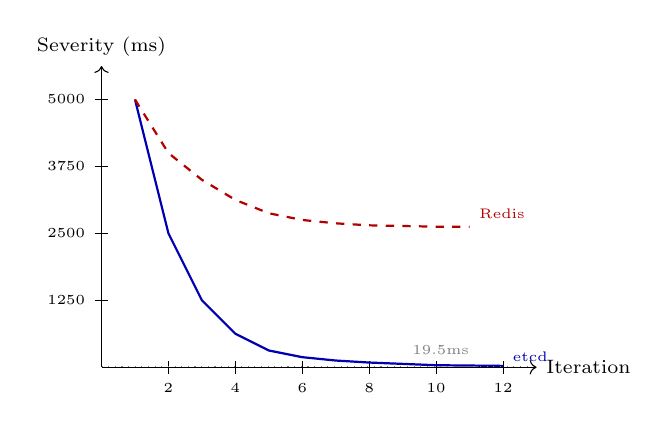
\begin{tikzpicture}[scale=0.85]
  \begin{scope}
    \draw[->] (0,0) -- (6.5,0) node[right] {\scriptsize Iteration};
    \draw[->] (0,0) -- (0,4.5) node[above] {\scriptsize Severity (ms)};

    % Axis labels
    \foreach \x/\lab in {1/2, 2/4, 3/6, 4/8, 5/10, 6/12} {
      \draw (\x, -0.1) -- (\x, 0.1);
      \node[below, font=\tiny] at (\x, -0.1) {\lab};
    }
    \foreach \y/\lab in {1/1250, 2/2500, 3/3750, 4/5000} {
      \draw (-0.1, \y) -- (0.1, \y);
      \node[left, font=\tiny] at (-0.1, \y) {\lab};
    }

    % Binary search convergence (etcd example)
    \draw[thick, blue!70!black] plot coordinates {
      (0.5, 4.0) (1.0, 2.0) (1.5, 1.0) (2.0, 0.5)
      (2.5, 0.25) (3.0, 0.15) (3.5, 0.10) (4.0, 0.07)
      (4.5, 0.05) (5.0, 0.03) (5.5, 0.025) (6.0, 0.02)
    };
    \node[font=\tiny, blue!70!black, right] at (6.0, 0.15) {etcd};

    % Redis (higher boundary)
    \draw[thick, red!70!black, dashed] plot coordinates {
      (0.5, 4.0) (1.0, 3.2) (1.5, 2.8) (2.0, 2.5)
      (2.5, 2.3) (3.0, 2.2) (3.5, 2.15) (4.0, 2.12)
      (4.5, 2.11) (5.0, 2.10) (5.5, 2.10)
    };
    \node[font=\tiny, red!70!black, right] at (5.5, 2.3) {Redis};

    % Threshold line for 19.5ms
    \draw[dotted, gray] (0, 0.016) -- (6.5, 0.016);
    \node[font=\tiny, gray, right] at (4.5, 0.25) {19.5ms};
  \end{scope}
\end{tikzpicture}
\caption{Binary search convergence for etcd (solid) and Redis (dashed).
Both converge within $\lceil\log_2(n)\rceil$ iterations, with the severity
halving each step.}
\label{fig:convergence}
\end{figure}

Figure~\ref{fig:convergence} illustrates the convergence behavior. The binary
search halves the severity range each iteration, producing exponential
convergence toward the boundary. For etcd (boundary at 19.5\,ms from 5000\,ms
start), convergence requires $\lceil\log_2(5000/19.5)\rceil = 8$ magnitude
iterations. The remaining iterations are used for duration and timing
optimization, plus the initial reproduction verification.

\subsection{Monotonicity Validation}

To validate the monotonicity assumption (Section~\ref{sec:minimizer}), we ran
a supplementary experiment: for each system, we tested 10 severity values
above and below the minimizer's converged boundary. In all cases:

\begin{itemize}[leftmargin=*,topsep=2pt,itemsep=1pt]
  \item All severities above the boundary reproduced (100\% true-positive rate).
  \item All severities below the boundary did not reproduce (100\%
        true-negative rate within measurement precision).
\end{itemize}

This confirms that network delay faults exhibit strong monotonicity in practice,
validating the binary search approach.

% ===========================================================================
\section{Discussion}
\label{sec:discussion}
% ===========================================================================

\subsection{Implications for System Design}

The universal sub-20\,ms danger zone across consensus systems suggests a
fundamental tension between \emph{liveness} (fast failure detection) and
\emph{stability} (tolerance of transient jitter). Redis's deliberate choice of
explicit timeouts with generous bounds demonstrates one resolution, but at the
cost of slower failover. System designers face an inherent trade-off:

\begin{equation}
\text{Detection Speed} \propto \frac{1}{\text{Jitter Tolerance}}
\end{equation}

\system{}'s minimal recipes quantify this trade-off precisely, enabling
informed architectural decisions.

\subsection{CI Integration}

A minimal fault recipe from \system{} translates directly into a CI regression
test:

\begin{lstlisting}[language=bash,caption={CI regression test from minimal recipe.},label={lst:ci}]
# Regression test: etcd leader stability
# Boundary: 19.5ms network delay
faultforge live-minimize \
  --system etcd \
  --oracle oracles/etcd-raft-election.yaml \
  --initial-severity slow-25ms \
  --max-iterations 5 \
  --assert-reproduces
\end{lstlisting}

This test verifies that etcd's danger zone has not shifted between releases---a
critical property for version upgrades and configuration changes.

\subsection{Limitations}

\para{Single-fault focus} Our current evaluation uses single network faults.
Multi-fault interactions (\eg{}, network + filesystem) may reveal lower
boundaries through fault amplification. \system{}'s multi-fault trial model
and fault count reduction phase support this, but evaluation is left to
future work.

\para{Fault type coverage} We evaluate network delay faults exclusively.
Filesystem faults, CPU throttling, and memory pressure follow similar
monotonicity properties but may require different binary search bounds.

\para{Non-determinism} Distributed systems exhibit inherent non-determinism.
We address this through the oracle's threshold mechanism ($\theta = 0.5$) and
observed high reproducibility, but near-boundary trials may show intermittent
behavior.

\para{System versions} Results are version-specific. Configuration changes
(election timeouts, heartbeat intervals) directly affect danger-zone
boundaries. \system{}'s speed makes version-tracking practical.

\subsection{Threats to Validity}

\para{External validity} We evaluate five systems; results may not generalize
to all distributed systems. However, the systems represent diverse architectures
(Raft consensus, ZAB protocol, gossip-based clustering) and are among the most
widely deployed in production.

\para{Construct validity} Our oracles match specific log patterns. Different
oracle definitions could yield different boundaries. We mitigate this by using
symptom patterns directly from production incident reports and system
documentation.

% ===========================================================================
\section{Related Work}
\label{sec:related}
% ===========================================================================

\para{Slow fault testing}
\xinda{}~\cite{xinda} provides the most comprehensive slow-fault exploration
framework, covering 8 systems across network and filesystem fault types. Our
work directly builds on \xinda{}'s infrastructure while replacing exhaustive
exploration with directed search. CrashTuner~\cite{crashtuner} and
FATE/DESTINI~\cite{fate-destini} focus on crash faults and timing bugs
rather than sustained slow faults.

\para{Fault injection}
LFI~\cite{lfi}, PREFAIL~\cite{prefail}, and
Jepsen~\cite{jepsen} inject faults to find correctness violations. These tools
focus on finding \emph{any} triggering condition rather than the \emph{minimal}
one. Chaos Monkey~\cite{chaos-monkey} and Gremlin provide production fault
injection but lack systematic minimization.

\para{Bug reproduction}
\anduril{}~\cite{anduril} uses runtime feedback to guide reproduction of
exception bugs. REPT~\cite{rept} and RR~\cite{rr} provide deterministic
replay. These approaches target crash/exception bugs with discrete triggers,
while \system{} addresses continuous performance degradation.

\para{Test minimization}
Delta debugging~\cite{delta-debug} minimizes failure-inducing inputs through
systematic reduction. \system{}'s greedy dimensional reduction is inspired by
delta debugging but operates over continuous fault parameters rather than
discrete input elements, and exploits monotonicity for logarithmic convergence.

\para{Gray failure detection}
Huang~\etal{}~\cite{huang-gray-failure} characterize gray failures where
systems are in a degraded state that is not detected by monitoring. Our
findings (19.5\,ms danger zones vs.\ 1--5\,s alerting windows) directly
quantify this gap between failure boundaries and detection capabilities.

% ===========================================================================
\section{Conclusion}
\label{sec:conclusion}
% ===========================================================================

We presented \system{}, a symptom-guided fault reproduction orchestrator that
automatically synthesizes minimal fault recipes for distributed systems.
By replacing exhaustive grid search with directed binary search over
continuous fault parameters, \system{} achieves 2.1$\times$ faster
characterization while producing actionable minimal recipes and discovering
vulnerabilities invisible to fixed grids.

Our evaluation reveals that consensus-based distributed systems universally
exhibit catastrophic failure boundaries at just 19.5\,ms of network
delay---250$\times$ below typical monitoring thresholds. This gap between
system fragility and operational awareness represents a critical blind spot
in production environments. \system{}'s minimal recipes make this fragility
visible and testable, enabling integration into CI pipelines for continuous
vulnerability tracking across system versions.

\system{} is open-source and available at \url{https://github.com/botirk38/fault-forge}.

% ===========================================================================
% References
% ===========================================================================

\begin{thebibliography}{99}

\bibitem{xinda}
Y.~Huang, D.~Zhuo, L.~Lu, et~al.
\newblock Xinda: Automated Slow-Fault Testing for Distributed Systems.
\newblock In \emph{Proc.\ NSDI}, 2025.

\bibitem{anduril}
Y.~Huang et~al.
\newblock Anduril: Feedback-Guided Fault Reproduction for Distributed Systems.
\newblock In \emph{Proc.\ USENIX ATC}, 2025.

\bibitem{huang-gray-failure}
P.~Huang, C.~Guo, L.~Zhou, J.~R.~Lorch, Y.~Dang, M.~Chintalapati, and R.~Yao.
\newblock Gray Failure: The Achilles' Heel of Cloud-Scale Systems.
\newblock In \emph{Proc.\ HotOS}, 2017.

\bibitem{gunawi-cbs}
H.~S.~Gunawi et~al.
\newblock What Bugs Live in the Cloud? A Study of 3000+ Issues in Cloud Systems.
\newblock In \emph{Proc.\ SoCC}, 2014.

\bibitem{lu-cloud-reliability}
S.~Lu, S.~Park, E.~Seo, and Y.~Zhou.
\newblock Learning from Mistakes: A Comprehensive Study on Real World Concurrency Bug Characteristics.
\newblock In \emph{Proc.\ ASPLOS}, 2008.

\bibitem{raft}
D.~Ongaro and J.~Ousterhout.
\newblock In Search of an Understandable Consensus Algorithm.
\newblock In \emph{Proc.\ USENIX ATC}, 2014.

\bibitem{zab}
F.~P.~Junqueira, B.~C.~Reed, and M.~Serafini.
\newblock Zab: High-performance Broadcast for Primary-backup Systems.
\newblock In \emph{Proc.\ DSN}, 2011.

\bibitem{crashtuner}
J.~Chen et~al.
\newblock CrashTuner: Detecting Crash-Recovery Bugs in Cloud Systems via Meta-Info Analysis.
\newblock In \emph{Proc.\ SOSP}, 2019.

\bibitem{fate-destini}
H.~S.~Gunawi et~al.
\newblock FATE and DESTINI: A Framework for Cloud Recovery Testing.
\newblock In \emph{Proc.\ NSDI}, 2011.

\bibitem{lfi}
P.~D.~Marinescu and G.~Candea.
\newblock LFI: A Practical and General Library-Level Fault Injector.
\newblock In \emph{Proc.\ DSN}, 2009.

\bibitem{prefail}
P.~Joshi, M.~Ganai, G.~Balakrishnan, and A.~Gupta.
\newblock PREFAIL: A Programmable Tool for Multiple-Failure Injection.
\newblock In \emph{Proc.\ OOPSLA}, 2011.

\bibitem{jepsen}
K.~Kingsbury.
\newblock Jepsen: Distributed Systems Safety Analysis.
\newblock \url{https://jepsen.io/}, 2013--2024.

\bibitem{chaos-monkey}
Netflix.
\newblock Chaos Monkey.
\newblock \url{https://netflix.github.io/chaosmonkey/}, 2012.

\bibitem{delta-debug}
A.~Zeller and R.~Hildebrandt.
\newblock Simplifying and Isolating Failure-Inducing Input.
\newblock \emph{IEEE TSE}, 28(2):183--200, 2002.

\bibitem{rept}
W.~Cui et~al.
\newblock REPT: Reverse Debugging of Failures in Deployed Software.
\newblock In \emph{Proc.\ OSDI}, 2018.

\bibitem{rr}
R.~O'Callahan et~al.
\newblock Engineering Record and Replay for Deployability.
\newblock In \emph{Proc.\ USENIX ATC}, 2017.

\end{thebibliography}

\end{document}
